\documentclass[preprint,12pt]{elsarticle}
\usepackage{graphicx}
\usepackage[margin=1.0in]{geometry}
\usepackage{color, colortbl}
\usepackage{hyperref}
\usepackage{float}
\usepackage{lineno}
\usepackage{tabularx} % For specifying table width
\usepackage{array}    % For additional column formatting options
%\linenumbers
% \usepackage[affil-it]{authblk}
\usepackage{subcaption}
\usepackage{listings}

\newcommand{\note}[1]{\textcolor{blue}{#1}}
\definecolor{LightCyan}{rgb}{0.88,1,1}
\definecolor{LightRose}{rgb}{1,0.88,0.88}
\definecolor{LightGreen}{rgb}{0.88,1,0.88}

\definecolor{codegreen}{rgb}{0,0.6,0}
\definecolor{codegray}{rgb}{0.5,0.5,0.5}
\definecolor{codepurple}{rgb}{0.58,0,0.82}
\definecolor{backcolour}{rgb}{0.95,0.95,0.92}

\lstdefinestyle{mystyle}{
    backgroundcolor=\color{backcolour},   
    commentstyle=\color{codegreen},
    keywordstyle=\color{magenta},
    numberstyle=\tiny\color{codegray},
    stringstyle=\color{codepurple},
    basicstyle=\ttfamily\footnotesize,
    breakatwhitespace=false,         
    breaklines=true,                 
    captionpos=b,                    
    keepspaces=true,                 
    numbers=left,                    
    numbersep=5pt,                  
    showspaces=false,                
    showstringspaces=false,
    showtabs=false,                  
    tabsize=2
}

\lstset{style=mystyle}

\title{High-Performance Data Format for Scientific Data Analysis}

\author[1]{Gagik Gavalian}
\address[1]{Jefferson Lab, Newport News, VA, USA}



\begin{document}

%\begin{titlepage}
\begin{abstract}
In this article, we present the High-Performance Output (HiPO) data format developed at Jefferson Laboratory for 
storing and analyzing data from Nuclear Physics experiments. The format was designed to efficiently store large
amounts of experimental data, utilizing modern fast compression algorithms. The purpose of this development was 
to provide organized data in the output, facilitating access to relevant information within the large data files. The HiPO
data format has features that are suited for storing raw detector data, reconstruction data, and the final physics analysis 
data efficiently, eliminating the need to do data conversions through the lifecycle of experimental data. The HiPO data format
is implemented in C++ and JAVA, and provides bindings to FORTRAN, Python, and Julia, providing users with the choice of data 
analysis frameworks to use.
In this paper, we will present the general design and functionalities of the HiPO library and compare the performance of the library with
 more established data formats used in data analysis in High Energy and Nuclear Physics (such as ROOT and Parquete).

\end{abstract}
%\end{titlepage}
\maketitle


\section{Introduction}

During past few years there was a big interest in using Artificial Intelligence (AI) in 
various ares of nuclear physics, from data processing to physics analysis. With continuously 
improving methods of Machine Learning (ML) and computational hardware it becomes easy to 
substitute some computational tasks with ML algorithms leading to smaller and computationally
more efficient code base. In this article we discuss implementation of Convolutional Auto-Encoders 
for de-noising data from CLAS12~\cite{Burkert:2020akg} tracking detectors (Drift 
Chambers~\cite{Mestayer:2020saf}). The de-nosing was used to analyze simulated data to measure
improvement on track reconstruction efficiency.

\section{Motivation}
\label{section-motivation}

%Data stored from physics experiments consists of "events" that record information from a setup for one interaction of the incident beam particle
%with the target. These "events" are processed independently to identify particles and tracks identified by different detector components and construct a physics event, which is then used for high-level physics analysis. The information stored in one "event" is a collection of responses from all detector components with unique data structures. The data collected during the experiment undergoes several transformations before it reaches the stage where it is used for physics analysis.

Physics experiment data consists of "events," each representing information captured from a single interaction between an incident beam particle and the target. These events are processed individually to identify particles and reconstruct tracks using data from various detector components. This process builds a complete physics event, which serves as the foundation for high-level physics analysis. Each event encapsulates a collection of responses from all detector components, organized in unique data structures. Before reaching the stage of physics analysis, the collected data undergoes multiple transformations to prepare and refine it for further study.

\begin{itemize}
\item The data acquisition records data from all detector components for one instance of interaction in raw format  (usually times and accumulated charge in each component of each detector system) 
\item In the next stage, the raw data is transformed from its digital form to values with units, such as time in milliseconds and energy in eV.
\item The reconstruction program analyses data from each detector to identify related signals and combines signals from various detectors to identify particles in each event (collision instance). The produced output contains tables with information about the particles in the event and the responses of each particle in each detector component, helping to identify particle species.
\item For each physics analysis, different sets of selection algorithms are used to identify the physics reaction in each event and physics observables are calculated based on detected particles in the event, and the output is produced containing a columnar table for final physics analysis. 
\end{itemize}

In traditional CLAS~\cite{CLAS:2003umf} experiments, different data formats were used at each stage of the data lifecycle, leading to unnecessary complexity. This required supporting multiple file formats and maintaining numerous conversion tools. Additionally, users developed dozens of data selection and filtering tools tailored to specific formats, all of which required ongoing maintenance. Initially, a similar approach was considered for the CLAS12~\cite{Burkert:2020akg} experiment during its early software development stages.

However, experienced developers quickly recognized the challenges of this approach and envisioned a more streamlined solution. To address these issues, it was decided to adopt a single data format for all stages of the experimental data lifecycle. Several existing formats, such as ROOT~\cite{Brun:1997pa}, LCIO~\cite{Aplin:2012kj}, and HDF5~\cite{HDF5:2000pa}, were evaluated. While each had its strengths, none were found to efficiently support all stages of data transformation. Furthermore, the growing diversity of data analysis frameworks and programming languages introduced additional challenges, as seamless integration required appropriate language bindings—complicating the use of existing formats in unified workflows.

To overcome these limitations, the High-Performance Output (HiPO)~\cite{hipo5p0:2025jk} data format was developed specifically for CLAS12. HiPO is designed to efficiently handle all stages of experimental data processing, from reconstruction workflows to final columnar data analysis. It also provides language bindings for a variety of programming languages used within the collaboration, including C++, FORTRAN, Python, Java, and Julia, ensuring broad compatibility and streamlined workflows.


To ensure usability across all workflows of data processing, several key requirements were established for the data format:

%Several requirements were imposed to ensure usability in all workflows of data processing, as follows:
\begin{itemize}
\item {\bf Serializable:} The CLAS12 reconstruction workflow follows a Service-Oriented Architecture (SOA) that operates on a heterogeneous platform using message passing. The data format was designed to be easily serializable, enabling efficient transmission of event data to individual reconstruction services.
\item {\bf Compression Efficiency:} To minimize storage demands, the data format incorporates compression. The compression algorithm must balance speed and compression ratio, as high compression speed is critical for managing the large data volumes produced by experimental setups, particularly in high-rate nuclear physics experiments where maintaining high data throughput is essential.
\item {\bf Random Access Capability:} The format must support random access to specific data collections within a file. This functionality is vital for debugging, selectively writing subsets of data, and supporting multi-threaded applications that process data chunks asynchronously.
\item {\bf Data Grouping Functionality:} The format should enable the grouping of related datasets, allowing for efficient tagging or marking of different datasets. This capability facilitates the targeted reading of specific groups without requiring the processing of the entire dataset.
\end{itemize}

The reconstruction of experimental data in CLAS12 is written in Java, for this reason, Java is the primary development platform of the HiPO library, and the C++ library is developed in parallel, sometimes lagging in features, but they are being slowly ported to the C++ code. Most of the example codes in this article are Java, the equivalent C++ examples can be found in the repository.
There are experimental bindings to Python and Julia, which are not actively developed due to limited use by collaborators.
The subsequent chapters will explore the features of the HiPO data format in greater detail, with illustrative examples.

\section{Design}

In nuclear physics experiments, data goes through multiple stages of transformation before reaching the physics analysis phase. Initially, raw signals are collected from the experimental setup, capturing the direct measurements from each detector component. These raw signals are then processed to extract key features, such as pulse shapes and timing information. 

The subsequent step involves integrating the data from individual detector components. Signals are grouped and correlated across detectors to identify matches, enabling the reconstruction of particle trajectories and characteristics. Finally, the reconstructed particles are analyzed to determine their interactions with each detector component, providing the foundation for further physics analysis.

%Conventionally, different data formats are used in different stages of the data lifecycle, which presents several challenges,
%maintaining a few different libraries for reading and writing files and maintaining code for translating between the data formats.
%This is using CPU cycles for just transforming data structures. Also, different data persistence libraries are using different compression algorithms with varying throughput and efficiency. 

Traditionally, different stages of the data lifecycle employ distinct data formats, which introduces several challenges. Maintaining multiple libraries for reading and writing files, as well as developing and maintaining code for translating between these formats, can be resource-intensive. This process consumes valuable CPU cycles solely for transforming data structures.

The use of diverse data persistence libraries, each employing unique compression algorithms, creates inconsistencies in throughput and efficiency. These variations complicate optimization efforts and can negatively impact the overall performance of data processing workflows.

This project aimed to design a unified data format capable of efficiently handling data across all stages of experimental workflows while facilitating the analysis of large datasets. The requirements for the new format were informed by extensive experience with experimental data and include the following:
\begin{itemize}
\item {\bf Compression Efficiency:} The data format must incorporate compression to minimize storage requirements. The chosen compression algorithm should strike a balance between speed and compression ratio. High compression speed is critical due to the large data volumes generated by experimental setups, particularly in high-rate nuclear physics experiments where high data throughput is essential.
\item {\bf Random Access Capability:} The format must support random access to specific data collections within a file. This feature is crucial for debugging, enabling selective writing of data subsets, and for multi-threaded applications that process chunks of data asynchronously.
\item {\bf Data Grouping Functionality:} The format should allow for the grouping of related datasets. This capability is essential for marking or tagging different datasets, enabling targeted reading of specific groups without the need to process the entire dataset.
\end{itemize}
For a more detailed explanation of these features and examples of their implementation, please refer to the following text.

\section{Format Description}

Data from physics experiments is organized into small units called "events," with each event containing data related to a single physics interaction captured by the detector. These events are collected over a certain period and stored sequentially in a file. A HiPO file, designed for this purpose, is structured into the following components:

\begin{figure}[h!]
  \begin{center}
    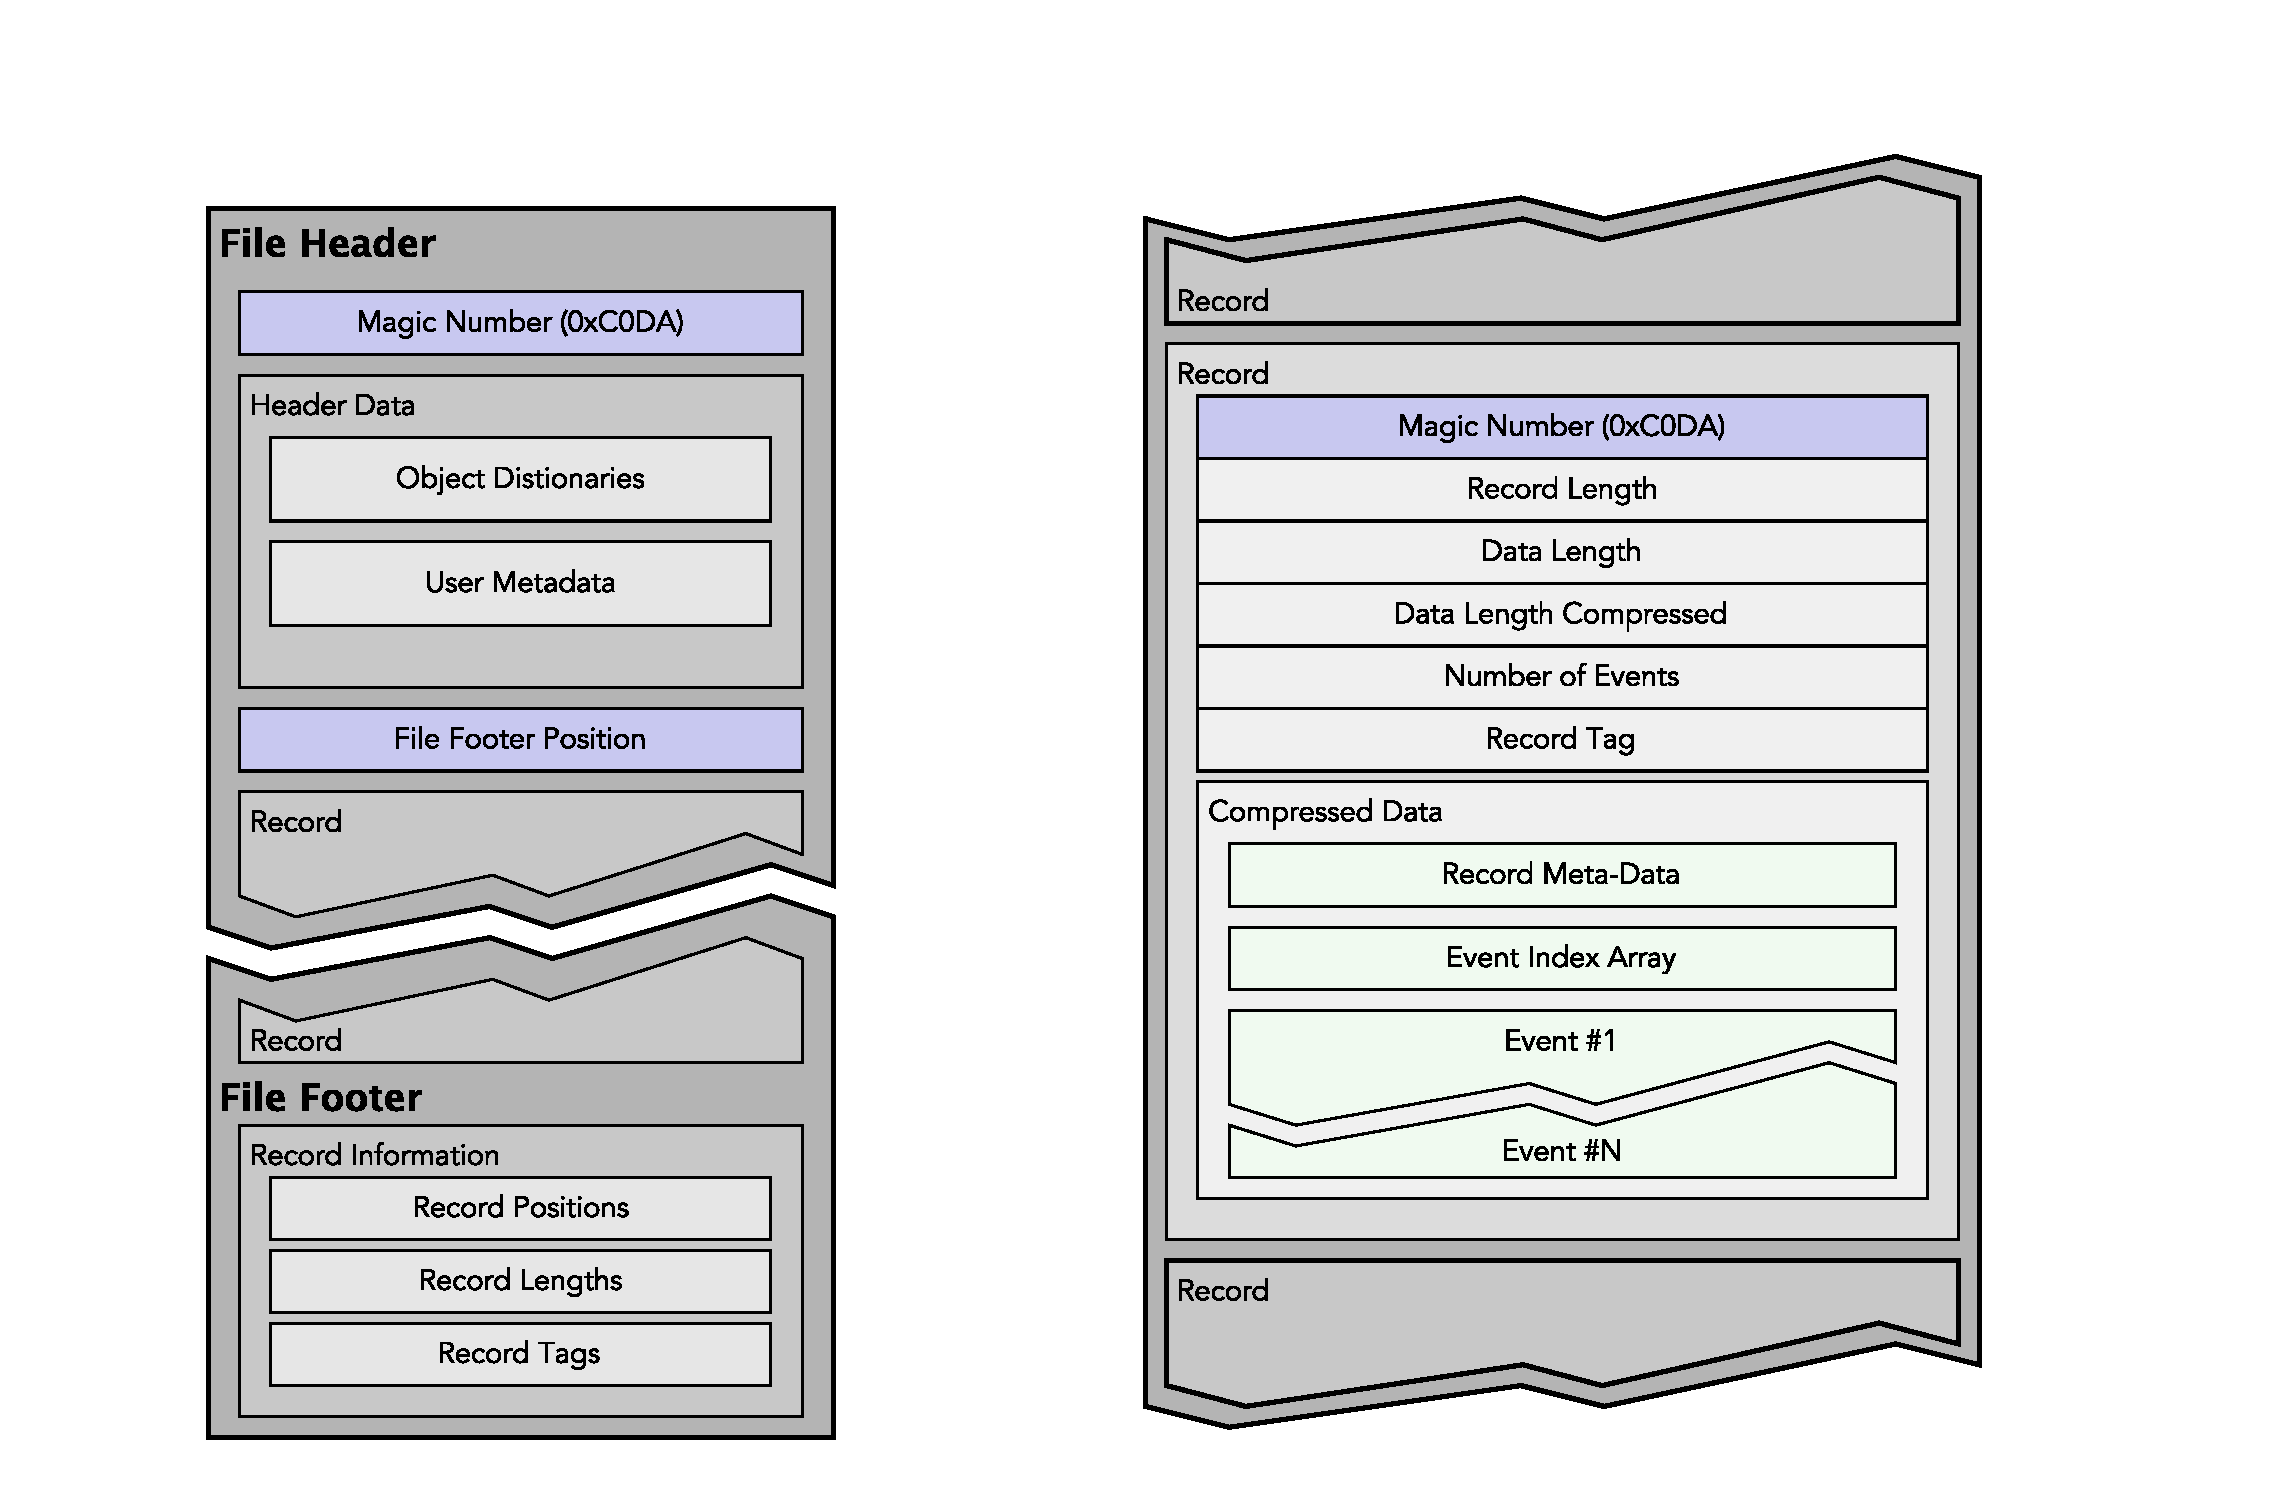
\includegraphics[width=0.85\textwidth]{images/file_structure.pdf}
 \end{center}
  \caption{Schematic view of the HiPO file structure. The figure shows the conceptual design of the file structure. It's not an exact layout of the data structures of the headers. The detailed documentation is published on the GitHub repository with the source code.}
 \label{schema:file}
\end{figure}


\begin{itemize}
\item {\bf File Header:} This section includes essential information such as the file version, file length (used for consistency checks), the location of the file footer, and other relevant parameters.
\item {\bf User Header:} This part contains metadata that describes the content of the file any other user provided metadata. In dictionary-driven formats, it includes descriptors (schemas for tabular data) of the data stored within the file.
\item {\bf Data Records:} These are the compressed, grouped data from individual events. The size of data records is configurable at the time of file creation. Each record is assigned a user-defined identifier, known as a tag, to group similar events together.
\item {\bf File Footer:} The footer contains metadata about each data record in the file, including its position, size, and tag.
The general structure of a HiPO file is illustrated in Figure~\ref{schema:file}.
\end{itemize}

The schematic view of the file structure is shown in Figure~\ref{schema:file}. 

\subsection{File Header}

The file header is a descriptor for the file containing information about the version of the file. This magic word identifies the file format and also carries information about the endianness of the data and the position of the file footer. The header also contains a block of data called "User Data". The user data includes dictionaries of the data objects stored in the file, as well as user-provided metadata describing the file or any parameters the creator may want to include with the file. This metadata comes in the form of key-value pairs usually provided by the user before the file initialization stage. To create a simple file with a given user header, use the code shown in Listing~\ref{lst:open_file}.
%\rule{16.5cm}{0.4pt}
\begin{lstlisting}[language=java, caption=Java example for writing a file with meta-data. The reader object opens the file and retrieves the stored mata data in a form of a key/value map., label=lst:open_file]
// -- open file with user-specified meta data
HipoWriter w = new HipoWriter(); // create the object
w.addConfig("date","created on 01/27/2021");
w.addConfig("author","John Pierce");
w.addConfig("type","Physics Events from A-Detector")
w.open("my_new_file.h5");
w.close();
// -- read metadata from the file
HipoReader r = new HipoReader("my_new_file.h5");
Map<String,String> userInfo = r.getUserConfigurations();
\end{lstlisting}


\subsection{Records}

The records contain data on events stored in sequence. The record header contains information on the number of events stored, an array of indices pointing to each of the events in the buffer, and the length of the data payload before compression and after the compression. The maximum size of the records for each given file is configured at the creation of the file, and the default size is $8~MB$. The record header also contains a unique identifier, which is "0" by default, and events that are added to the file are recorded in sequence in the 
record until the record size limit is reached, at which point the record is compressed and persisted on the disk with the record header attached, and the record is cleared to start receiving the next events. This process continues until the file is closed, at which point the file footer is recorded, containing positions and identifiers of the records. The file header is updated with the position of the file footer for fast access when opening the file for reading.

\subsection{Events}

As it was mentioned above, the HiPO file consists of a series of events. An event is one unit containing a bunch of data objects that are related to each other. The types of data that can be stored in the event are arrays of primitive types and tables. Each object is assigned two identification numbers, which are used to 
retrieve these objects at the read. These identifiers are called "group" (16 bits) and "item" (8 bits). These logical identifiers can be used to group relevant data, use your imagination. The primitive types are simple arrays, and their headers describe the data structure unequivocally and they do not require dictionaries to be read. 

\subsubsection{Primitive types}

The primitive types are arrays of numbers and strings where all elements of the array have the same type (such as byte, short, integer, float, double, long, and string). The objects 
called Node are created from a provided array with user-defined identifiers. The example Listing~\ref{lst:write_arrays} shows how to create their primitive arrays and how to write them into an event:
\rule{16.5cm}{0.4pt}
\begin{lstlisting}[language=java, caption=Java example to create and write primitive types into an event, label=lst:write_arrays]
// Writing arrays into an Event
Event event = new Event(2048); // creta event with max size 2 kB
float[]  df = new float[]{1.0,2.0,3.0,4.0};
short[]  ds = new short[]{3,5,8,13,21,34,55};
Node   nf = new Node(12,1,df);
Node   ns = new Node(12,2,ds);
Node data = new Node(12,3,"Event recorded at 12:52:33"); 
event.write(nf);
event.write(ns);
event.write(data);
\end{lstlisting}

It's worth noting that the preliminary size of the event does not restrict the user to write objects that exceed the allocated event size. As new objects are added to the event, the event buffer 
will adopt the necessary size to accommodate the objects. It is recommended to set the size slightly larger than is needed to avoid reallocations for better performance.

\subsubsection{Tables}

Tables are rectangular data structures with columns and rows. Table objects require a schema (a descriptor) to be able to parse the content. The schema must be created 
and declared before the file is opened for writing since the file writer composes a dictionary and stores all schemas in the header of the file. The data structure that holds
tables is called a Bank and is also assigned two unique identifiers (group, item). The Listing~\ref{lst:write_bank} shows a simple example of how to declare and write a 
simple bank into a file:
\rule{16.5cm}{0.4pt}
\begin{lstlisting}[language=java, caption=Java example to create and write banks (tables) into an event, label=lst:write_bank]
// Writing banks to the event
SchemaBuilder b = new SchemaBuilder("data::clusters",12,1)
    .addEntry("type","B","cluster type") // B - type Byte
    .addEntry("n", "S", "cluster multiplicity") // S - Type Short
    .addEntry("x", "F", "x position") // F - type float
    .addEntry("y","F","y position") // F - type float
    .addEntry("z", "F", "z position"); // F - type Float
// -- create a cchema
  Schema schema = b.build();
// add schema to the file and open the file
  HipoWriter w = new HipoWriter();
  w.getSchemaFactory().addSchema(schema);
  w.addConfig("date","file created at 11:54:22 AM");
  w.addConfig("description","file contains clusters in calorimeter");
  w.open("clusters.h5");                
  Event event = new Event();
  Bank  b  = new Bank(schema,2); // create a table with 2 rows
  b.putByte("type", 0, (byte)   1); b.putByte("type", 1, (byte)   2);
  b.putShort("n"  , 0, (short) 13); b.putShort("n"  , 1, (short) 21);
  b.putFloat("x",0,0.1f); b.putFloat("x",1,0.2f);
  b.putFloat("y",0,1.1f); b.putFloat("y",1,1.2f);
  b.putFloat("z",0,2.1f); b.putFloat("z",1,2.2f);
  event.write(b);
  w.addEvent(event);
  w.close(); // close should be called to write the file footer
\end{lstlisting}

The methods to write and read values for each element in the bank have two interfaces, one using the name of the variable
which makes for more readable code, and the second method using the index of the column which provides better performance 
when needed. The same setters can be used as follows, b.putFloat("x",0,0.1f) $\rightarrow$ b.putFloat(2,0,0.1f), since "x" is the third 
column in the table (column indices are counted starting from "0"). The correct types of setters have to be used when writing the data 
to ensure that the values provided do not overflow the boundaries of the type. However, more generic getters can be used when reading 
the data, such as $getInt(entry, row)$ for all integer types and $getDouble(entry, row)$ for all floating point types.

\rule{15.5cm}{0.4pt}
\begin{lstlisting}[language=java, caption=Java example to read banks from the file, label=lst:read_bank]
HipoReader r = new HipoReader("clusters.h5");        
Bank[] banks = r.getBanks("data::clusters");
// to read more than on bank use: r.getBanks("a","b","c","d");
// If the bank is not present in the event, the returned object 
// will have getRows()==0, no error is generated.
while(r.nextEvent(banks)){
  System.out.printf("\%4d, \%5d, \%8.5f \%8.5f \%8.5f\n",
           banks[0].getInt("type", row),
           banks[0].getInt(1,row),
           banks[0].getFloat("x", row),
           banks[0].getFloat("y", row),
           banks[0].getFloat("z", row));
}
\end{lstlisting}

In Listing~\ref{lst:read_bank} shows how to read the banks from a file and print the content on the screen. The 
$getBanks(String... list)$ method accepts a list of the banks to be read in each event, so multiple banks can be
read and analyzed at once. More advanced examples of how to read events and query the content of the events 
can be found in the examples provided in the repository.

The Listing~\ref{lst:read_bank} provides a simple reading procedure when the banks are automatically read for each event 
for the user. The more complex code can be found in the repository where the Event object is read from the file and then
banks can be read individually from the event, deleted and/or augemented and written into output. 

%\begin{figure}[h!]
%  \begin{center}
%   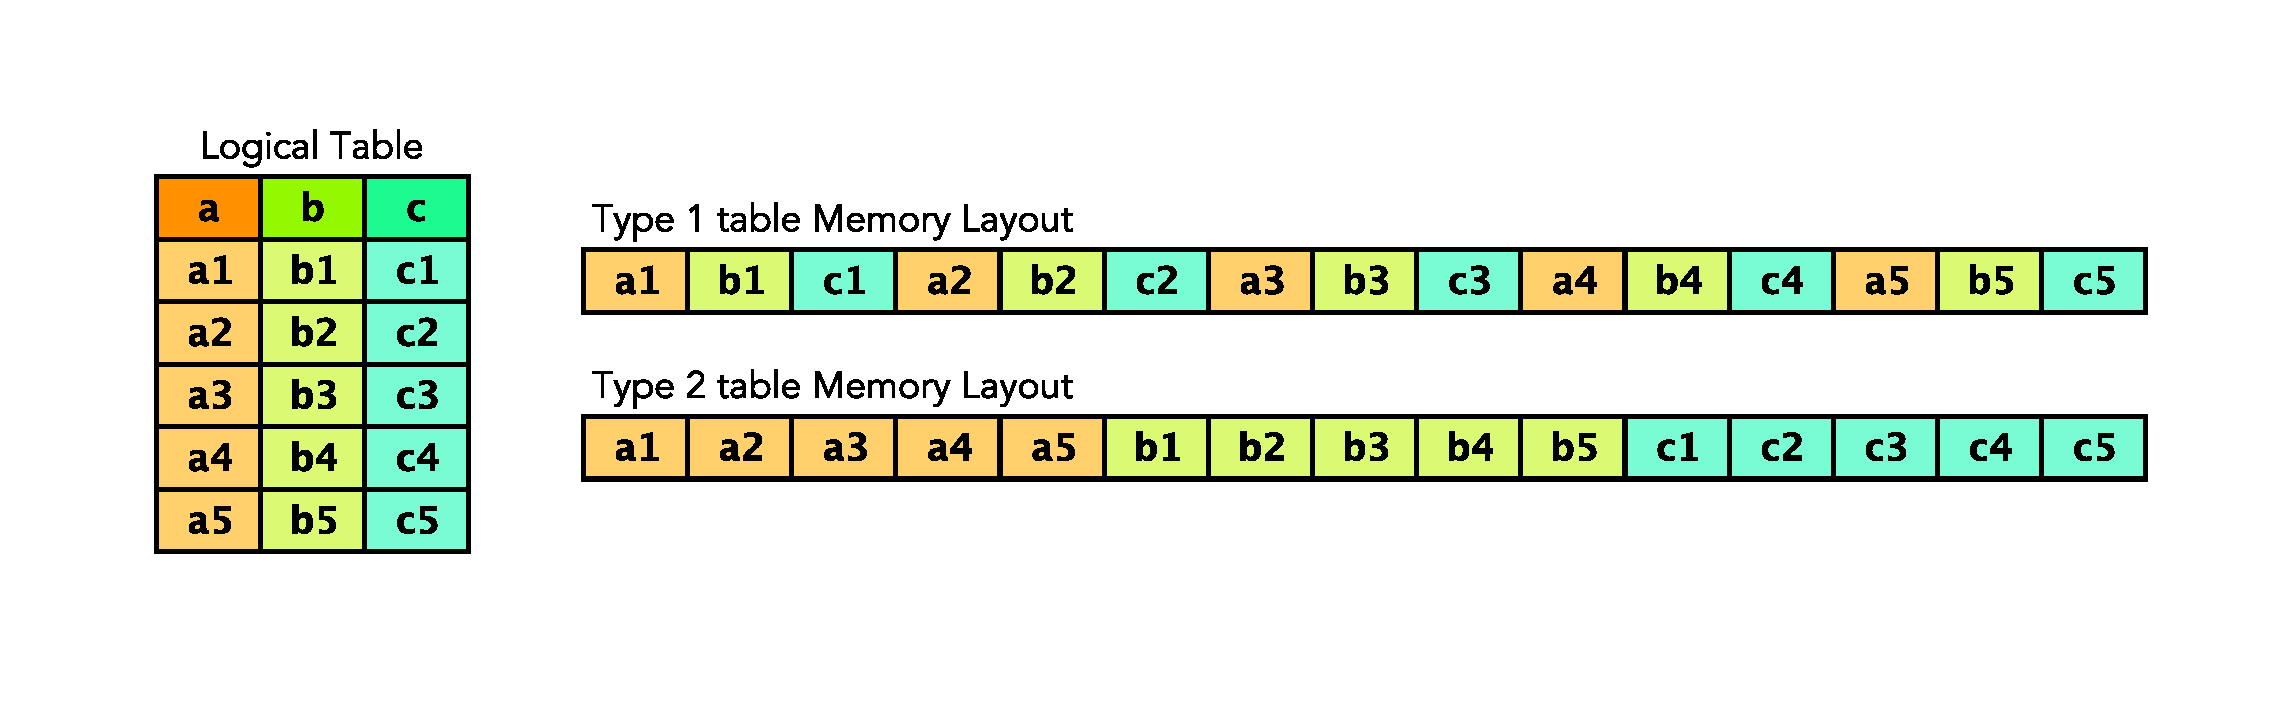
\includegraphics[width=0.95\textwidth]{images/table_layouts.pdf}
% \end{center}
%  \caption{Table types with their memory layout. Type 1 tables are optimized for copying and deleting rows from the table without much overhead on copying individual bytes, while Type 2 tables are better for compression, proving $7\%-15\%$ reduction in the bank size.}
% \label{fig:table_layouts}
%\end{figure}

%The HiPO provides two types of tables where the rows and columns are arranged differently. In the example above
%each column from all the rows is grouped together into a contiguous memory, which makes it necessary to declare 
%the number of rows at the bank creation time and the banks' size can not be changed on the fly. The second type
%is when each row is one contiguous memory block and rows can be altered on the fly, which makes it easy to manipulate
%rows programmatically by removing a row or copying a row into an equivalent table. The schematic view of memory
%mapping for these two types of tables is shown in Figure~\ref{fig:table_layouts}. The reason for having two types of
%tables is that one (the case with columns forming a contiguous memory) is better for data compression which makes
%it more efficient for producing final data sets for analysis. The second table type is used for workflows where different
%components work on the same data set that analyzes the tables by appending and removing entries from a given bank.
%In the particular case of experimental physics usage is the data acquisition system, where a table is growing with incoming
%data, and some rows are removed based on some conditions imposed by the analysis software. In our workflows, the table
%where column values are grouped provides $7\%-15\%$ more compression. Examples of how to use different types of tables
%can be found the the code repository.



%Example usages:
%\begin{verbatim}
%hipo::writer writer("output.file");
%for(int i = 0; i < 12000; i++){
%   hipo::event event = event_provider_next();
%    writer.addEvent(event);
%}
%writer.close();
%\end{verbatim}



%The data from physics experiments is stored in small units called "events", each event contains data related to one physics interaction from a detector. The file consists of a series of events accumulated by the experimental setup during a certain period of time. A HiPO file consists of the following parts:

%- File header: containing file version file length (for consistency check), file footer location, and some other relevant parameters.
%- User header: contains metadata describing the content of the file. In dictionary-driven content contains descriptors of the data 
%stored in the file, the user can add additional information at the creation of the file.
%- Data records: The actual event data grouped and compressed. The size of the data records is configurable at the file creation time. Each record is assigned a user-defined identifier (called tag), which is used to group similar events together.
%- File footer: Contains information about each record in the file, including position, size, and the tag of the record.
%A general structure of the HiPO file is shown in Figure~\ref{hipo_file_structure}.


\section{Event Tagging}

The HiPO is designed to store data in units of events, where events are collections of data related to each other (usually in time). In nuclear physics
experiments, these events refer to one interaction of a beam particle with the target and record particles produced by the interaction. After the data 
acquisition, the post-processing of the data identifies the number of particles produced and their properties and writes them in the event for further
physics analysis. Specific interactions occur with different frequencies in the physics experiment, and the analysis program analyzing specific physics 
reactions does not analyze every single event but rather requires a specific number of produced particles reconstructed to proceed with the analysis.

In Figure~\ref {fig:event_frequency}, a schematic view is shown of how data can be theoretically distributed in the file. Where event types, are defined by 
a number of rows in the table that lists the particles reconstructed by data processing software. It is evident that for analysis of rare interactions, most of
the data read is not useful and the program spends unnecessary I/O cycles putting pressure on a shared file system and computational resources.

\begin{figure}[h!]
  \begin{center}
    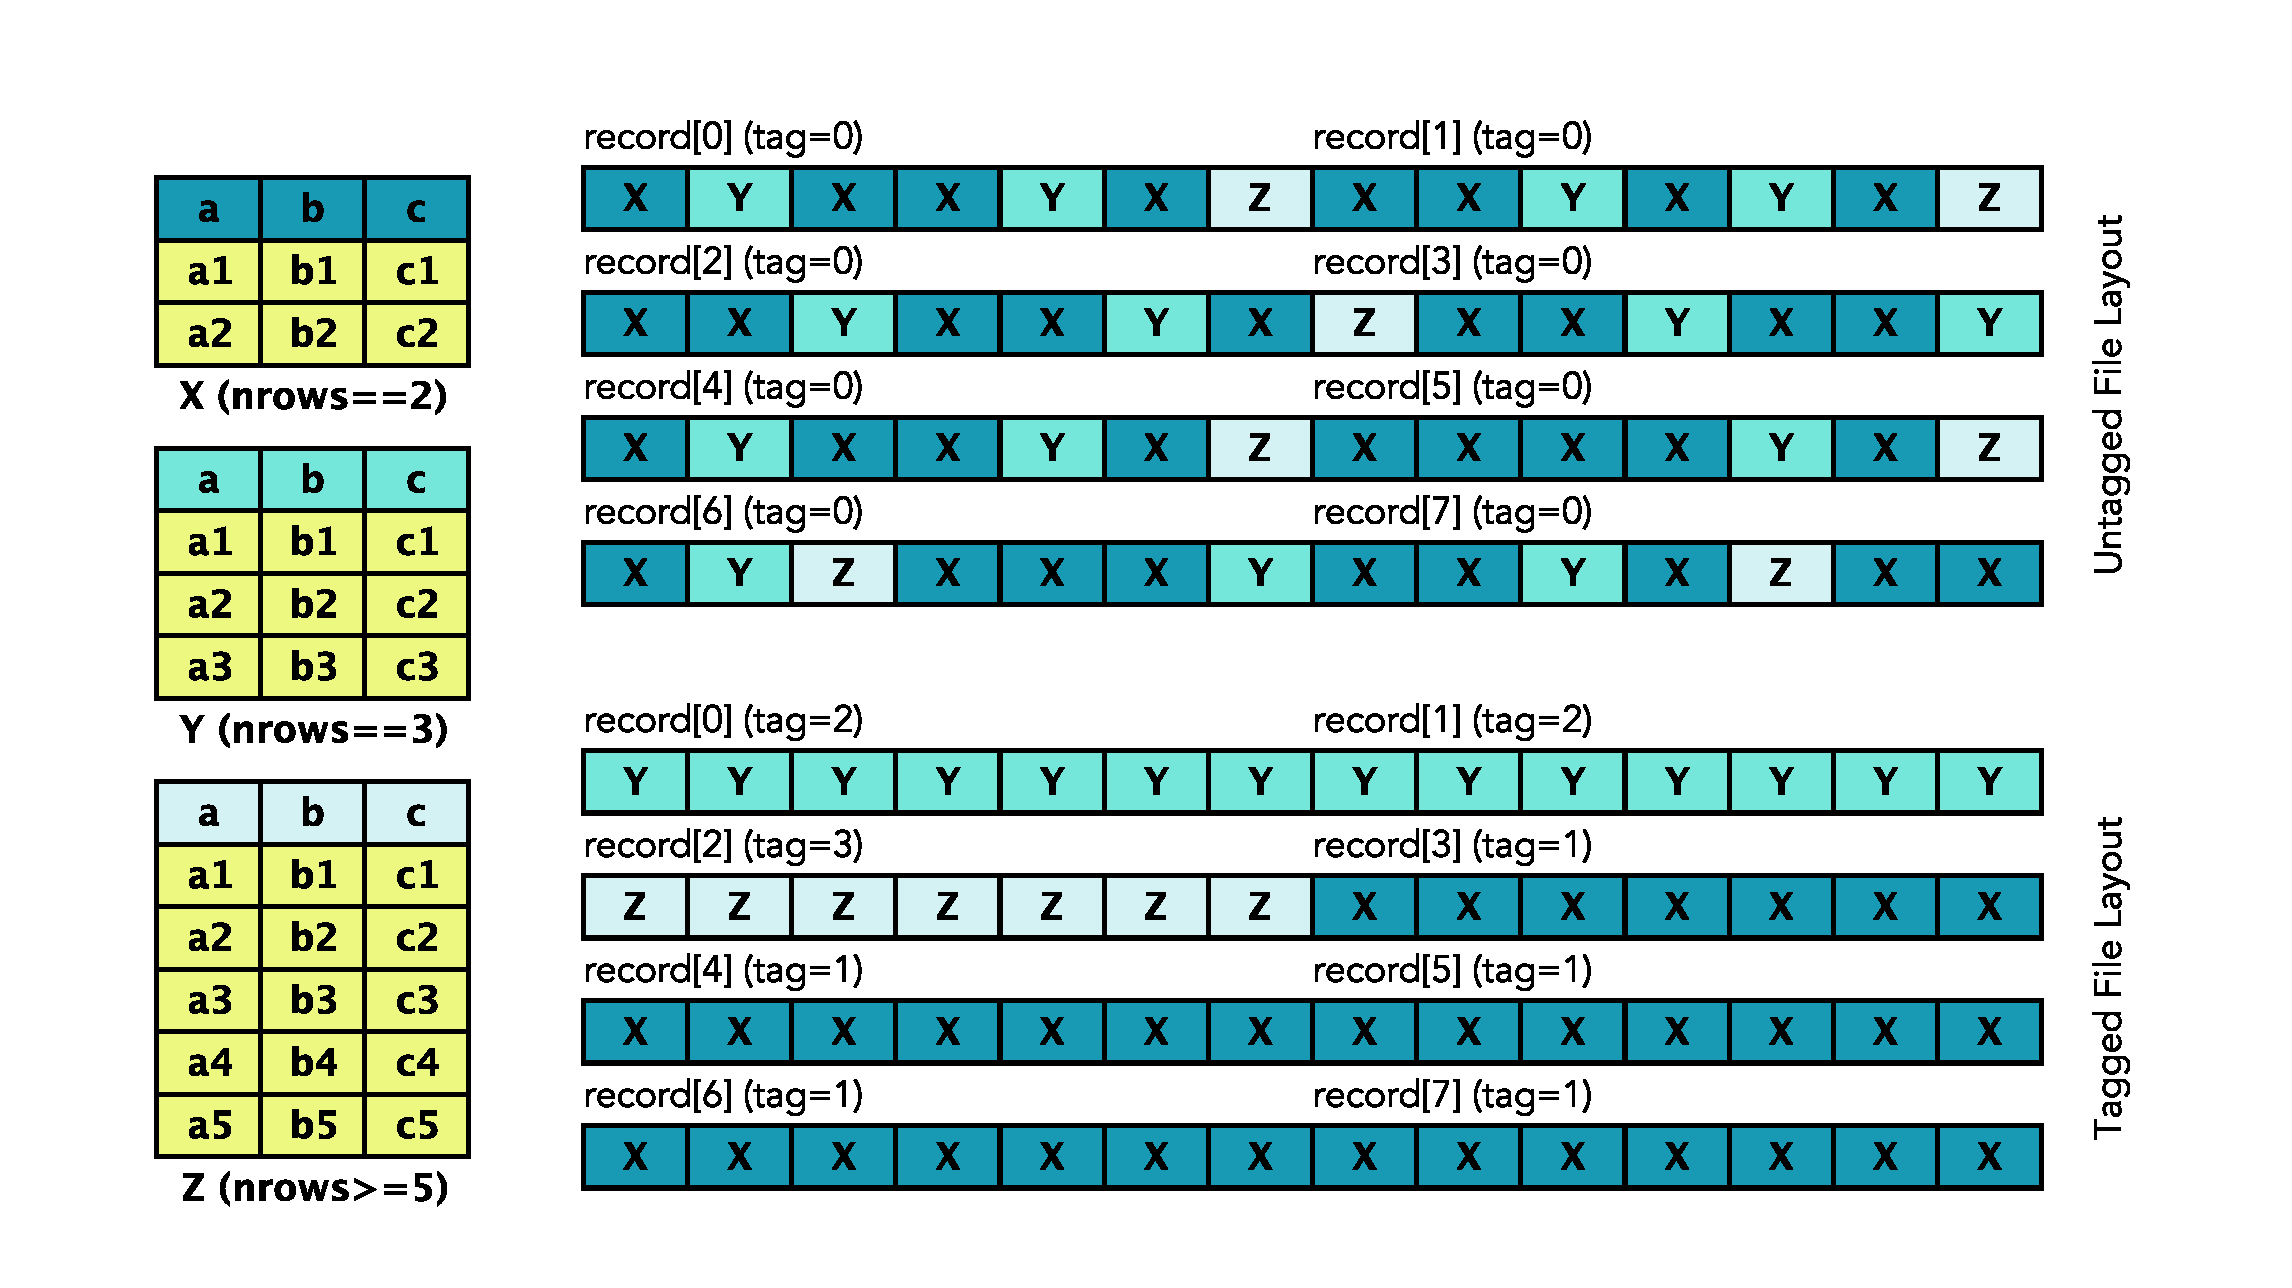
\includegraphics[width=0.85\textwidth]{images/tagged_records.pdf}
 \end{center}
  \caption{Schematic view of the file output for tagged and untagged events. When using the tagged mode of writing a file, events are organized in the records 
  based on the tag of the event, which is assigned by the user depending on the needs.}
 \label{fig:event_frequency}
\end{figure}

To solve this problem, the HiPO data format introduces a tagging feature for storing data. As mentioned before, each record kept in the file contains a unique
tag identifier and this information is stored in the file footer along with the record's positions and sizes. This allows sorting events into separate records during
the writing of the file, which will organize similar events together. The Listing~\ref{lst:write_tagged} shows an example of how to tag events by the number of 
rows contained in a table that lists clusters from the previous example. 

\rule{16.5cm}{0.4pt}
\begin{lstlisting}[language=java, caption=Java example to create and write primitive types into an event, label=lst:write_tagged]
// Writing arrays into an Event
HipoReader r = new HipoReader("myfile.h5");
// using HipoWriter.create() transfers all the dictionary
// and the metadata to the write object
HipoWriter w = HipoWriter.create("taggedfile.h5",r);

Bank[] b = r.getBanks("data::clusters");
Event event = new Event();
while(r.next(event)){
  event.read(b);
  if(b[0].getRows()>=5){
      event.setTag(5);
  } else {
  	event.setTag(b[0].getRows());
  }
  w.addEvent(event);
}
w.close();
\end{lstlisting}

The example code with produce a file where all events with a matching number of rows are grouped together. the events with a specific number of
rows in the "clusters" bank can be read without any overhead of going through the entire file, and example of reading events where the number of
rows in the "clusters" bank are equal to 2 or are larger than 4 as shown in Listing~\ref{lst:read_tagged}.

\rule{16.5cm}{0.4pt}
\begin{lstlisting}[language=java, caption=Java example to sort events in the output file depending on number of rows in the table, label=lst:write_tagged]
// Writing arrays into an Event
HipoReader r = new HipoReader();
r.setTags(2,5); // read only tag=2 and tag=5
r.open("taggedfile.h5");
Bank[] b = r.getBanks("data::clusters");
while(r.nextEvent(b)){
   b[0].show();// print bank content on the screen
}
\end{lstlisting}

Only the bank "data::clusters" containing two rows and/or more than four rows is read in the Listing~\ref{lst:write_tagged}, however, then the event is written to the output file and the entire event with all the banks and nodes is written, but the decision on how to partition a file is based only on one bank. 




%Example usages:
%\begin{verbatim}
%hipo::writer writer("output.file");
%for(int i = 0; i < 12000; i++){
%   hipo::event event = event_provider_next();
%    writer.addEvent(event);
%}
%writer.close();
%\end{verbatim}



%The data from physics experiments is stored in small units called "events", each event contains data related to one physics interaction from a detector. The file consists of a series of events accumulated by the experimental setup during a certain period of time. A HiPO file consists of the following parts:

%- File header: containing file version file length (for consistency check), file footer location, and some other relevant parameters.
%- User header: contains metadata describing the content of the file. In dictionary-driven content contains descriptors of the data 
%stored in the file, the user can add additional information at the creation of the file.
%- Data records: The actual event data grouped and compressed. The size of the data records is configurable at the file creation time. Each record is assigned a user-defined identifier (called tag), which is used to group similar events together.
%- File footer: Contains information about each record in the file, including position, size, and the tag of the record.
%A general structure of the HiPO file is shown in Figure~\ref{hipo_file_structure}.


\section{Columnar Data Storing}

The final stage of any data analysis is representing the data in a columnar format and fetching some subset of the data with constraints 
on other columns. At this stage, users operate on a large data set with many columns and rows, and access to all of the 
columns in the file is not required. The Apache Parquet format is widely used in data science for storing columnar data, due to its tools
with Python data frames. It is highly tuned to store large data sets and provide fast access to required columns. The Parqute is gaining
some popularity in High Energy and Nuclear Physics with the growing popularity of Python as a physics analysis environment. In the
past two decades, the ROOT was the primary tool for physics analysis which also provides data structures for storing columnar data 
and accessing the columns selectively. It is worth mentioning that ROOT also has Python bindings. 

\subsection{Design}

The flexibility of the HiPO data format allows storing data in columnar format, similar to Parquete and ROOT. 
The feature of assigning tags to records allows for writing the data in a columnar manner, where each column is assigned a tag and written separately into its own record.
This process is synchronized so that at every predetermined number of rows, every column data is serialized and outputted as a record. The schematic view of arranging 
the data in the file is shown in Figure~\ref{fig:tuple_schema}.

\begin{figure}[h!]
  \begin{center}
    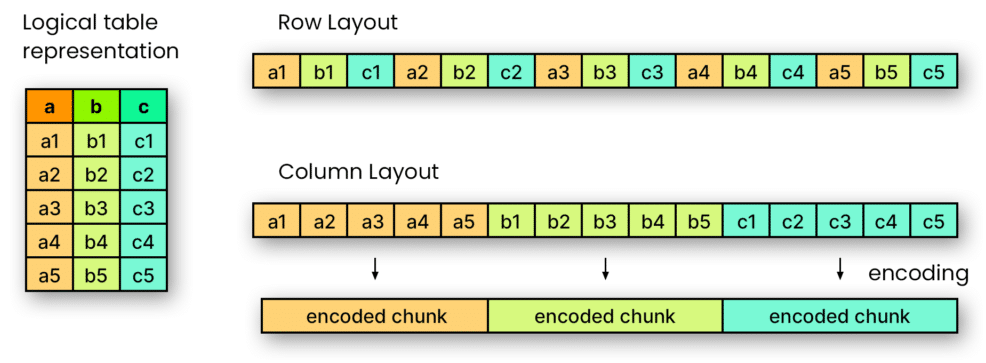
\includegraphics[width=0.85\textwidth]{images/tuple_schema.png}
 \end{center}
  \caption{Schematic view of arranging each event in the file from columnar table.}
 \label{fig:tuple_schema}
\end{figure}

When reading the file, the desired columns (called branches) are declared, and only records (buckets) with corresponding tag numbers are read and deserialized.
The user program has access only to the declared branches. The files written as columnar data have to be read with the corresponding API to make sure that the columns 
are properly synchronized at the read time. Here is an example code to read a few columns from a file and fill histogram. 
%\begin{verbatim}
\rule{16.5cm}{0.4pt}
\begin{lstlisting}[language=c++, caption=c++ example to read tuple file and fill histogram.]
// open file and read only specified branches
hipo::tuple tuple("tuple.h5", "c1:c2:c3:c4"); 
float data[4]; // declare a holder for the data to be read
twig::h1d h(120,-1.0,1.0); // declare a histogram
while(tuple.next(data)==true){
    h.fill(data[0]);
}
\end{lstlisting}
%\end{verbatim}

The example code code opens a file to read branches names "c1"-"c4" from the file, reads all rows until reaching the end of the file passing them to the user code through a declared array.
The values from the first branch (which is "c1") will be filled into a histogram.

\subsection{Benchmarking}

For reading tests, we produced a synthetic data set consisting of 24 columns and 50 M rows and created HiPO (4.8 GB), ROOT (4.4 GB), and Parquete (5.1 GB) all three with 
LZ4 compression. The columns were filled with random numbers generated by the Java Random class with a Gaussian distribution with a standard deviation of 1.0. 

\begin{figure}[h!]
  \begin{center}
    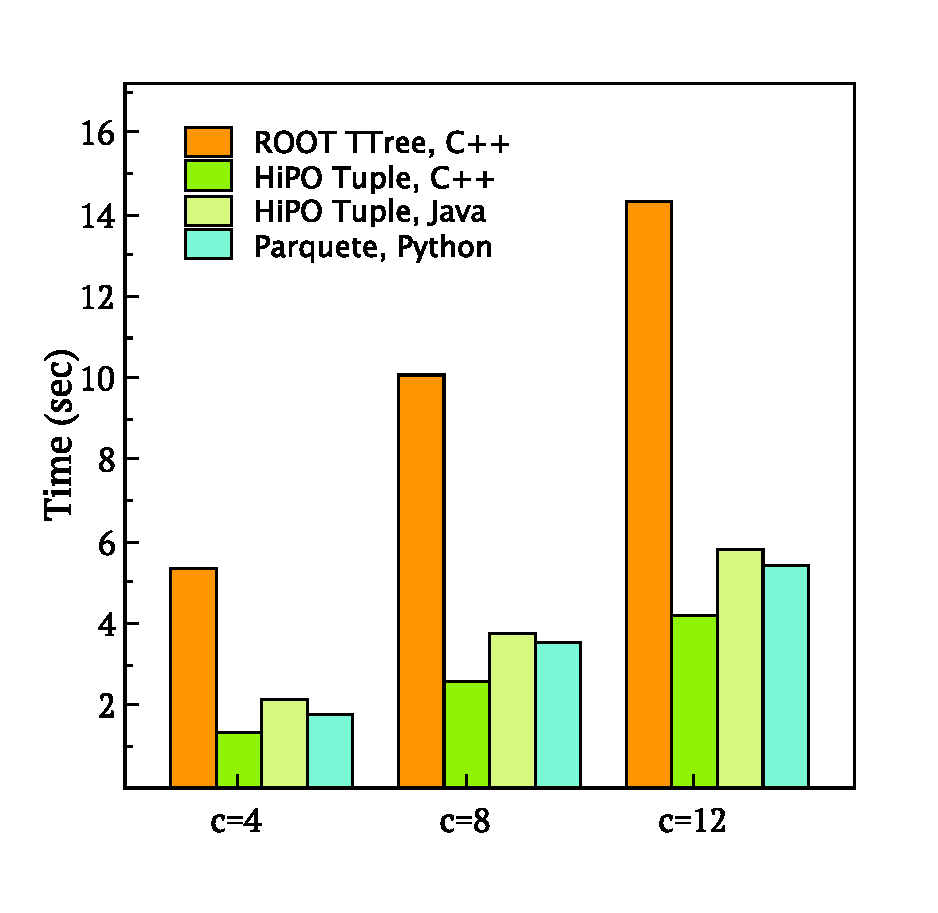
\includegraphics[width=0.45\textwidth]{images/read_benchmark.pdf}
     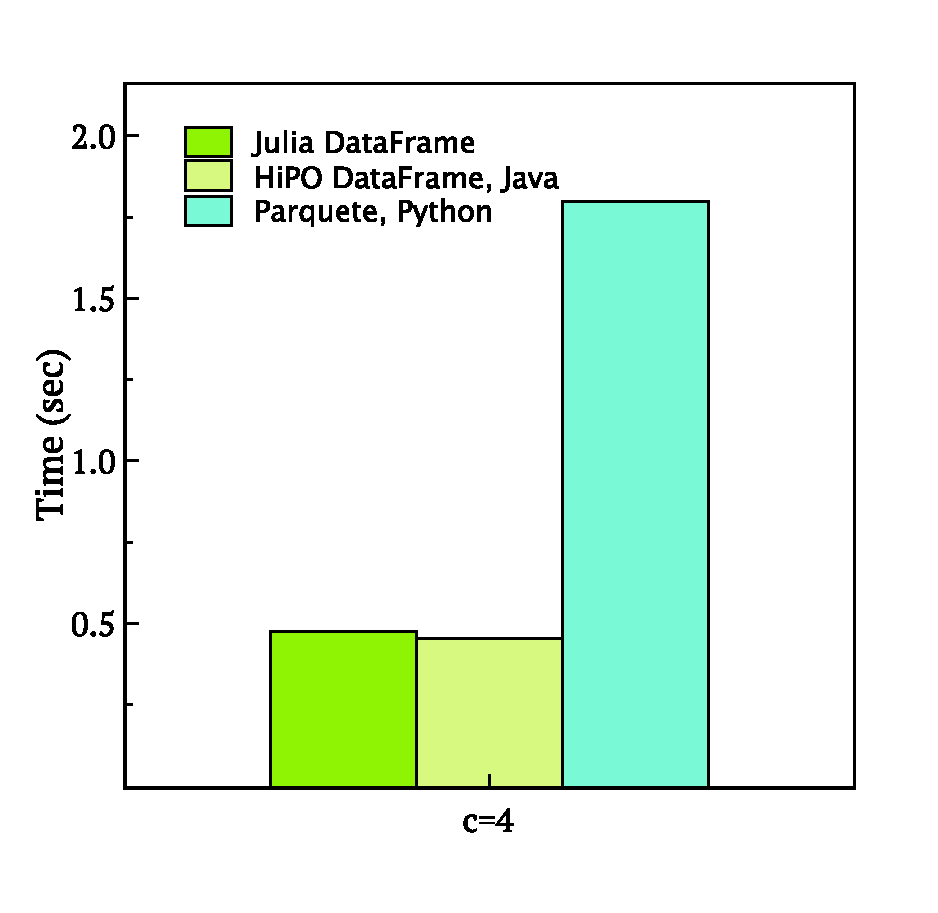
\includegraphics[width=0.45\textwidth]{images/data_frame_benchmark.pdf}
 \end{center}
  \caption{Reading benchmark for different file formats reading the same data with 24 columns and 50 M rows. Nd - is the number of columns that are read from the file, and a histogram is filled for each column. }
 \label{read_benchmark}
\end{figure}

Then, reading tests were performed by reading 4, 8, and 12 branches (out of 24) from the data file and filling a histogram for each branch, representing a typical workflow for data exploration. The times were measured for ten consecutive reads, and the average time of the last four reads was used as the final result. The results are shown in Figure~\ref{read_benchmark}. As can be seen from the figure the ROOT TTree has the worst performance. The C++ HiPO library has the best read times, followed closely by Parquete. Surprisingly the Java HiPO library is very close to Parquete in performance. 


\begin{table}[h!]
\centering
%\begin{tabular}{|l|c|c|c|c|} % '|' for borders, 'c' for center alignment
\begin{tabular}{|p{4cm}|p{1.5cm}|p{2cm}|p{2cm}|p{2cm}|p{2cm}|}
\hline
\textbf{Format (Library)} & Size  & write (sec) & c=4 & \textbf{c=8} & \textbf{c=12}  \\ \hline \hline
ROOT TTree (C++)  &  4.4 GB & 106.40 & 5.37 sec&10.10 sec& 14.35 sec       \\ \hline
HiPO Tuple   (C++)   & 4.8 GB & -  & 1.35 sec & 2.61 sec & 4.22 sec       \\ \hline
HiPO Tuple  (Java)   & 4.8  GB & 5.82 & 2.16 sec & 3.78 sec & 5.84 sec     \\ \hline
Parquete (Python)     &  5.1 GB & 15.97 & 1.80 sec & 3.56 sec & 5.44 sec        \\ \hline
DataFrames (Julia)   &  4.8 GB & - & 0.48 sec & 0.70 sec & 0.96 sec      \\ \hline
DataFrames  (Java)   & 4.8  GB & 5.82 & 0.35 sec & 0.53 sec& 0.57 sec   \\ \hline
DataFrames  (C++)   & 4.8  GB & 5.82 & 0.55 sec & 0.73 sec& 0.94 sec   \\ \hline
\end{tabular}
\caption{Reading benchmark for different file formats reading different numbers of columns from the file with 24 columns and 50 M rows, and filling histograms for each read column. Nd - is the number of columns read from the file, and a histogram is filled for each column. At the time of writing this article, the tuple files can be written only in Java, a command line tool exists for importing a CSV file. The DataFrames, in this work, for C++ and Java refer to the custom implementation of simple data frames that allow cycling through data and filling histograms in one bulk call. }
\label{tab:read_benchmark}
\end{table}

The numerical reading values for these tests are summarized in Table~\ref{tab:read_benchmark}. It is important to note that the writing performance of the data format is very important if it will be used in online for storing the experimental data. The faster serialization is preferable for the choice of data format. The writing times for the different formats are also summarized in Table~\ref{tab:read_benchmark}, and as it can be seen the writing times for HiPO are significantly shorter compared to both ROOT and Parquete.

The benchmarks are performed on a M1 Macbook Laptop with a 1 TB SSD drive.

\section{Discussion}

So it goes.



\newpage

\section{Acknowledgments}

This material is based upon work supported by the U.S. Department of Energy, Office of Science,
Office of Nuclear Physics under contract DE-AC05-06OR23177, and NSF grant no. CCF-1439079 and
the Richard T. Cheng Endowment. This work was performed using the Turing and Wahab computing
clusters at Old Dominion University.
 
 
\begin{thebibliography}{}
%\cite{Aplin:2012kj}
\bibitem{Brun:1997pa}
R.~Brun and F.~Rademakers,
``ROOT: An object oriented data analysis framework,''
Nucl. Instrum. Meth. A \textbf{389} (1997), 81-86
doi:10.1016/S0168-9002(97)00048-X
\bibitem{Aplin:2012kj}
S.~Aplin, J.~Engels, F.~Gaede, N.~A.~Graf, T.~Johnson and J.~McCormick,
``LCIO: A Persistency Framework and Event Data Model for HEP,''
doi:10.1109/NSSMIC.2012.6551478

\bibitem{HDF5:2000pa}
The HDF Group,  http://www.hdfgroup.org/HDF5/

%\cite{Brun:1997pa}

%3821 citations counted in INSPIRE as of 08 Jan 2025
%12 citations counted in INSPIRE as of 08 Jan 2025
\end{thebibliography}
%\newpage
%\bibliography{references}
%\bibliographystyle{ieeetr}

\end{document}
